\section{Our Framework \mname{}}


Formally, we are given a corpus of training utterances $\mathcal{D_T}$ labeled with $S$ seen intents, and a corpus of unlabeled utterances $\mathcal{D_C}$ consisting of $U$ novel intents such that $S \cap U = \varnothing$. We propose a three-stage framework \mbox{\mname{}} that (i) classifies the incoming test utterance $x \in \mathcal{D_C}$ with one of the $S = (s_1, ..., s_S)$ seen intent labels or as an \textit{unseen} (\textit{novel}) intent; (ii) for utterances $\mathcal{D_X}$ predicted as having a novel intent, it discovers the latent intents $U = (u_1, ..., u_U)$ present in them; and (iii) links together mutually related novel intents discovered to form novel domains, and an intent-domain taxonomy. %We now describe these three stages of \mname{} below.


\subsection{Stage I: Detecting Instances with Novel Intents}
\label{sec:stage1}

We construct a two-step system to detect instances with \textit{novel} intents, inspired by the success of models pre-trained on large unlabeled corpora, like GPT~\cite{radford2018improving} and BERT~\cite{devlin2018bert}. 

\smallskip
\noindent \textbf{Step I:} 
Prior open classification literature has modeled the problem of finding \textit{novel} or \textit{unseen} classes as an $(S+1)$-class  classification problem, with $S$ \textit{seen} classes and an additional \textit{unseen} class. Labeled training data is available for the seen classes, and an input instance is classed as unseen if it does not belong to any of the seen classes~\cite{xu2019open,shu2018unseen,shu2017doc}. 
In a similar vein, to classify utterances as containing a novel intent or not, we learn a BERT based multi-class classifier (Figure~\ref{fig:stage1}). 
Given an input utterance $\bm{x}$, it is converted into a sequence of tokens to be input to BERT. A special classification embedding \texttt{[CLS]} is added as the first token. %, and another special token \texttt{[SEP]} is used for separating segments. The input representation is a concatenation of WordPiece embeddings~\cite{wu2016google}, positional embeddings, and the segment embedding. 
The output of BERT is an $n$-dimensional utterance encoding $(\bm{e_1},...,\bm{e_n})$. A multi-class intent classification layer on top of BERT predicts the utterance intent based on the final hidden state $\bm{e_1}$ of the \texttt{[CLS]} token as: 

\begin{center}
$y = \textrm{softmax}(\bm{W e_1} + \bm{b})$
\end{center}

\noindent where $\bm{W}$ is a task-specific parameter weight matrix. 
%Intuitively, the lower layer of the BERT model may contain more general information than the higher layers. 
We fine tune the parameters $\theta$ in different BERT layers with different learning rates as in~\cite{howard2018universal}, %. We split the parameters $\theta$ to be tuned into ${\theta_1, \theta_2, ..., \theta_L}$, where $\theta_l$ contains the parameters of the $l$-th layer of BERT. The parameters are then updated 
as follows:

\begin{center}
$\theta_t^l = \theta_{t-1}^l - \eta^l \nabla_{\theta_l} J(\theta)$
\end{center}

\noindent where $\eta_l$ and $\theta_l$ represent the learning rate and parameters respectively of the $l$-th BERT layer. $\nabla_{\theta_l} J(\theta)$ is the gradient with respect to the model's objective function. We set the base learning rate to $\eta^L$ and use $\eta^{l-1} = \xi.\eta^l$, where $\xi$ is a decay factor $\leq$ 1. %When $\xi < 1$, lower layers have a lower learning rate than higher layers. %When $\xi = 1$, all layers have the same learning rate, which is equivalent to the regular stochastic gradient descent (SGD). 
We fine-tune all BERT parameters as well as $\bm{W}$ jointly by maximizing the log-probability of the correct intent label.
%More details about these parameters are given in the Evaluation section.

%As part of training data for our multi-class classification model described above, we use the data consisting of utterances labeled with seen intents ($\mathcal{D_T}$). %However, unlike previous approaches, in order to classify an utterance $x$ as belonging to an unseen or novel intent, we utilize the following two sets of heuristics: 

For our $(S+1)$-class classification model described above, labeled training data $\mathcal{D_T}$ is available for the $S$ seen intents. We use \textit{out-of-domain} (OOD) intent detection datasets distinct from both $\mathcal{D_T}$ and $\mathcal{D_C}$, as training data for the $(S+1)$-th `novel' intent class. This OOD data comes from out-of-domain intent-labeled publicly available datasets (e.g. SNIPS~\cite{coucke2018}, ATIS~\cite{dahl1994}). Since we use already annotated, publicly available intent labeled data as OOD data, we don't require extra human annotation effort here. Note that while training, \mname{} only requires the information that the OOD intents do not overlap with those in $\mathcal{D_T}$ or $\mathcal{D_C}$, and \textit{not} the actual intent labels of the OOD data. 
However, if the OOD data is annotated with $m$ intent classes, \mname{} can use this information by fragmenting the $(S+1)^\text{th}$ class into $m$ classes, forming an $(S+m)$-class classification layer. Using $m$ classes may provide a better representation of the utterances likely to contain unseen intents (as shown in Section~\ref{sec:evalution}). An utterance classified into any of the $m$ classes is flagged as having a novel intent. 
% consisting of $m$ different intent classes. These OOD datasets can be any intent-labeled data that does not contain intents present in the $\mathcal{D_T}$ or $\mathcal{D_C}$ corpora. 
%If a test utterance is classified into any of the $m$ classes, we flag it as containing a novel intent. 

\smallskip
\textbf{Step II:} \mname{} employs an additional check as per the DOC algorithm~\cite{shu2017doc}. DOC learns statistical confidence thresholds for each seen intent class $s_i$. DOC thus captures instances that have been classified to one the $S$ seen intents with a low confidence. 
If the class-specific prediction probabilities for an input utterance are less than the thresholds learned for each seen intent $s_i$, that utterance is also classified as having a novel intent (see Figure~\ref{fig:stage1}). 


%\begin{itemize}

%\item We formulate our multi-class classification layer in Figure~\ref{fig:stage1} with $(S+m)$ intent class labels, for $S$ seen intents and $m$ possible novel or unseen intents. If a test utterance is classified into any of the $m$ classes, we flag it as containing a novel intent. As training data for the $m$ unseen intents, we use labeled data from \textit{out-of-domain} (OOD) datasets consisting of $m$ different intent classes. These OOD datasets can be any intent-labeled data that does not contain intents present in the $\mathcal{D_T}$ or $\mathcal{D_C}$ corpora. 

%\item We employ an additional check as per the DOC algorithm~\cite{shu2017doc} for those utterances that are classified as belonging to a seen intent with a confidence score below a learned threshold. DOC learns class-specific statistical confidence thresholds for each intent class. If the class-specific prediction probabilities for a test instance are less than their respective class thresholds, the instance is considered to contain a novel intent. 
%\end{itemize}


%A multi-class intent classification layer on top of BERT predicts the utterance intent. 

%\noindent The above approach categorizes all test utterances as containing either a seen or a novel intent.


\begin{figure}
\begin{subfigure}{.45\textwidth}
  \centering
  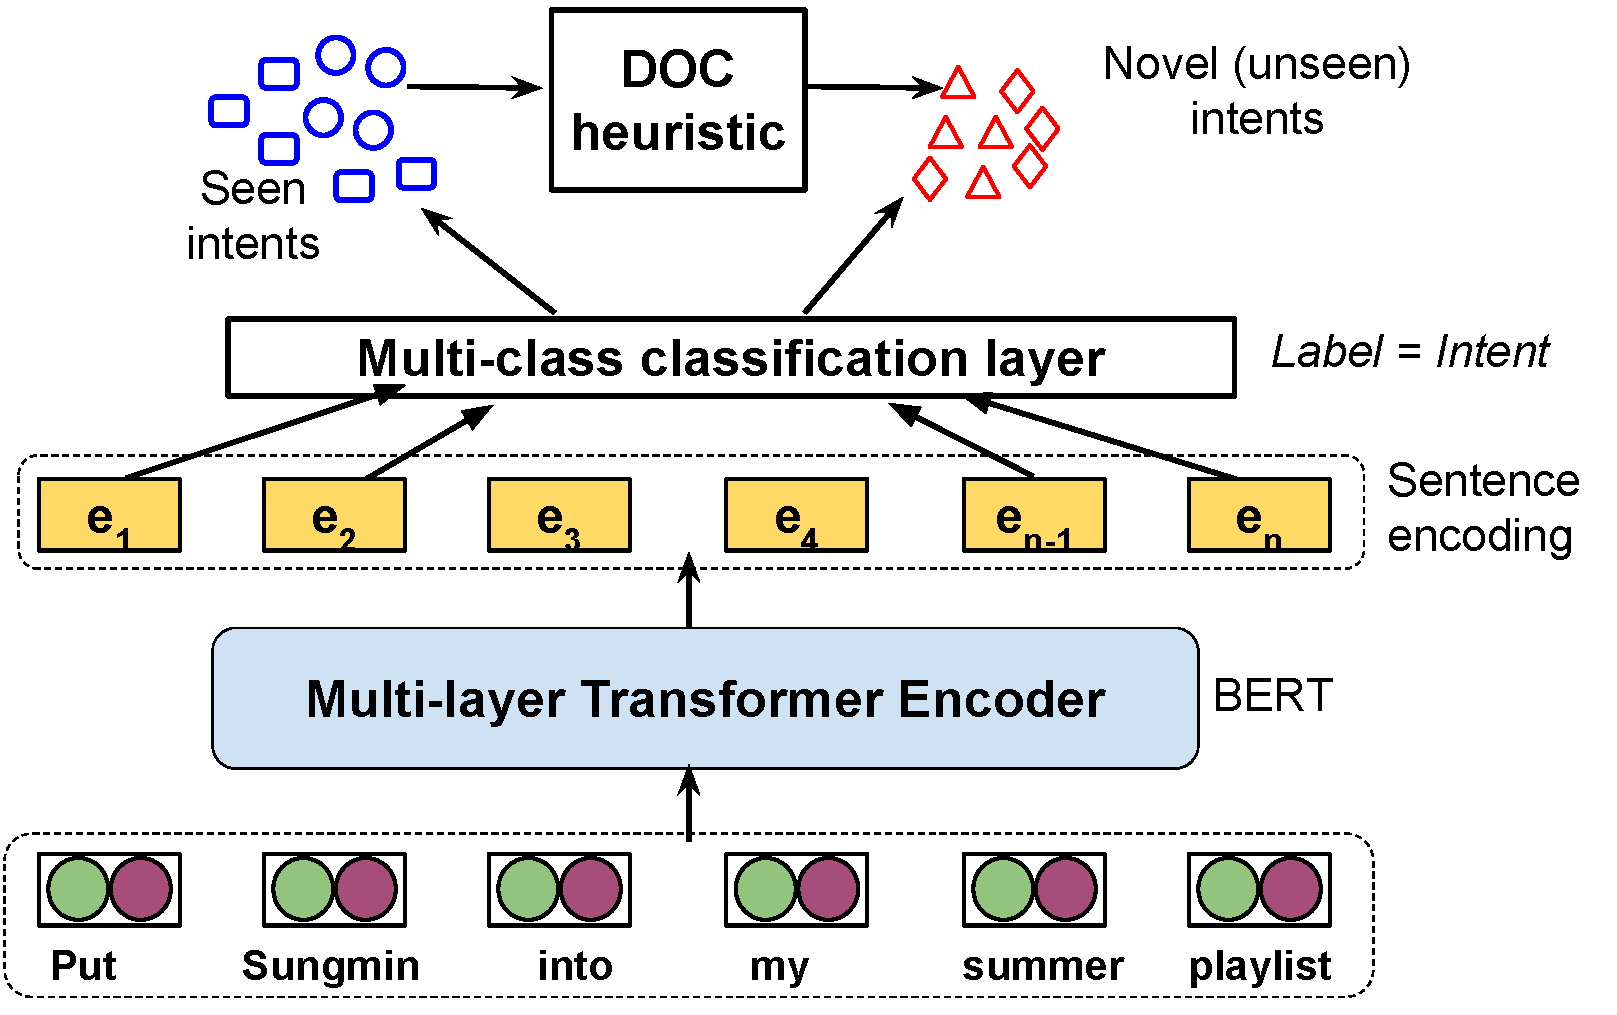
\includegraphics[height=4cm]{stage1}
  \caption{Detecting instances containing novel intents}
  \label{fig:stage1}
\end{subfigure}%
\begin{subfigure}{.45\textwidth}
  \centering
  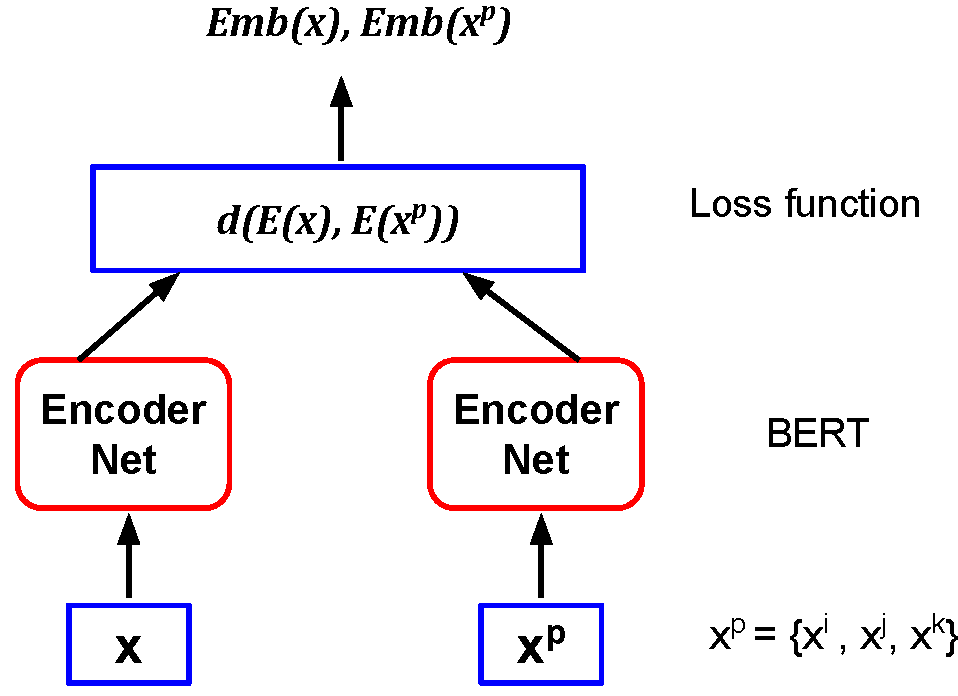
\includegraphics[height=4cm]{stage2}
  \caption{Discovering Novel Intent Categories}
  \label{fig:stage2}
\end{subfigure}
\caption{Overview of both stages of our approach, \mname{}}
\label{fig:advin}
\end{figure}



\subsection{Stage II: Discovering Novel Intent Categories}
\label{sec:stage2}

The output of the previous step of \mname{} gives us all utterances $\mathcal{D_X}$ that potentially contain a newly emerging intent. The next step is to discover the actual latent intent categories $U$ within $X$. We use complete-linkage, agglomerative hierarchical clustering~\cite{gowda1978agglomerative} to group together related utterances in $\mathcal{D_X}$, and find the potential novel intents $U$. %Starting with each utterance as a cluster, pairs of clusters are successively merged based on the distance between them. The merging stops when a certain maximum distance $\delta$ between clusters is reached. 

\smallskip

\noindent \textbf{Knowledge Transfer Component: }
Intuitively, humans seem to understand and categorize newly encountered objects based on the characteristics of similarities or differences that they learn from their prior knowledge of similar or comparable objects. We utilize a similar idea in order to learn the distance threshold $\delta$ for hierarchical clustering. That is, we transfer the knowledge learned from clustering the utterances containing seen intents $S$, to the utterances containing novel intents.
First, we perform hierarchical clustering on the labeled training data utterances $\mathcal{D_T}$, using the seen intents as ground truth cluster labels. %Starting with each utterance as a cluster, pairs of clusters are successively merged based on the distance between them. The merging stops when a certain maximum distance $\delta$ between clusters is reached. 
We obtain a distance value that maximizes the inter-intent distance between utterance clusters and minimizes the intra-intent distance within a cluster, by maximizing the F1 score of their clustering arrangement. 
In an ideal scenario, every obtained cluster $L_i$ represents a single seen intent. We also assume that utterances in the training set $\mathcal{D_T}$ of seen intents, as well as those in the unlabeled corpus $\mathcal{D_X}$ of newly emerging unseen intents come from similar distributions. %We can therefore transfer the distance threshold knowledge learned from clustering the seen intents to the novel or unseen intents. 
Our final step is then to \textit{transfer} this distance threshold $\delta$ learnt from the \textit{seen} intent utterances, to hierarchically cluster utterances in $\mathcal{D_X}$ containing novel or unseen intents. The distance threshold $\delta$ is defined as $\max\limits_{x \in L_i, x^p \in L_j} f(Emb(\bm{x}), Emb(\bm{x^p}))$ according to complete-linkage hierarchical clustering. Here, function $f(.)$ quantifies the distance between the embeddings $Emb(.)$ of an utterance pair $(\bm{x}$, $\bm{x^p})$ belonging to clusters $L_i$ and $L_j$ respectively.  %Hierarchical clustering stops when the distance $\delta$ between clusters is reached. 
%The value of $\delta$ for a clustering arrangement of the labeled training utterances $\mathcal{D_T}$ is the largest distance $dist(L_i, L_j)$ between every pair of clusters $L_i$ and $L_j$, and is given by: %$dist(C_i, C_j)$ is given by:

%\begin{center}
%$\delta = max_{i \neq j} dist(C_i, C_j)$
%\end{center}

%\noindent where $dist(C_i, C_j)$ is the distance between a pair of clusters $C_i$ and $C_j$, and is given by:


%\begin{center}
%\[
 %   dist(L_i, L_j) = \max\limits_{x \in L_i, x_p \in L_j} f(Emb(\bm{x}), Emb(\bm{x_p}))
%\]  

%\end{center}

%\noindent $f(Emb(\bm{x}), Emb(\bm{x_p}))$ denotes a distance function between the embeddings of a pair of utterances $\bm{x}$ and $\bm{x_p}$ (from Figure~\ref{fig:stage2}). These distances are given as input to the hierarchical clustering algorithm. 
We now describe how we learn the distance function $f$ between pairs of utterances.

\begin{comment}
\begin{figure}[t]
\centering

\includegraphics[width=0.95\columnwidth]{Figures/stage2} % Reduce the figure size so that it is slightly narrower than the column. Don't use precise values for figure width.This setup will avoid overfull boxes. 
\caption{Discovering Novel Intent Categories}
\label{fig:stage2}
\end{figure}
\end{comment}

\smallskip

\noindent \textbf{Learning Pairwise Utterance Distances for Clustering: }
We learn a neural network model to obtain utterance embeddings $Emb(.)$ for both the labeled corpus of seen intents ($\mathcal{D_T}$) and the unlabeled utterances detected to have novel intents ($\mathcal{D_X}$). %Figure~\ref{fig:stage2} displays the proposed architecture of our model. 
To train this model (see Figure~\ref{fig:stage2}), we create a training dataset from $\mathcal{D_T}$ comprising pairs of utterances $(x, x^p)$. Both $x$ and $x^p$ contain a seen intent. For each $x$, there are three possible choices for its paired utterance $x^p$: (i) $x^i$ containing the same domain and intent as $x$, (ii) $x^j$ containing the same domain but different intent than $x$, and (iii) $x^k$ containing a different domain and intent than $x$. Thus, $x^p \in \{x^i, x^j, x^k\}$. 
These utterance pairs $(x, x^p)$ are fed as input to an \texttt{EncoderNet}, which consists of a BERT transformer block. We use the same learning rate decay strategy of fine-tuning the BERT layers as earlier. Representations $E(\bm{x})$ and $E(\bm{x^p})$ are learned by the second last BERT layer (Figure~\ref{fig:stage2}).
The next layer on top of the \texttt{EncoderNet} blocks uses a distance function $d$ to compute pairwise representation distances, subject to the following bi-directional constraints: (i) the distance $d(E(x), E(x^i))$ between the representations of $x$ and $x^i$ should be less than $d(E(x), E(x^j))$; (ii) $d(E(x), E(x^i))$ between the representations of $x$ and $x^i$ should be less than $d(E(x), E(x^k))$; and (iii) the distance $d(E(x), E(x^j))$ between the representations of $x$ and $x^j$ should be less than the distance $d(E(x), E(x^k))$ between the representations of $x$ and $x^k$. These constraints utilize the semantic relationships between the utterance pairs containing different types of seen domains and seen intents. 
%Thus the next layer uses a distance function $d$ to compute the representation distances and enforce these constraints, which 
We then formulate a loss function $\mathfrak{L}$ to train our model, given by:

%\begin{center}
%$d(E(x), E(x^i)) + m_1 < d(E(x), %E(x^j))$
%$d(E(x), E(x^i)) + m_2 < d(E(x), %E(x^k))$
%$d(E(x), E(x^j)) + m_3 < d(E(x), %E(x^k))$
%\end{center}

\begin{align*}
%\mathfrak{L} &= \frac{1}{M} \sum\limits_{i, j, k} \{\max[0, m_1 + d(E(x), E(x^i)) - d(E(x), E(x^j)] \\ 
& \frac{1}{M} \sum\limits_{i, j, k} \{\max[0, m_1 + d(E(x), E(x^i)) - d(E(x), E(x^j)] + \alpha \max[0, m_2 + d(E(x), E(x^i)) - d(E(x), \\
& E(x^k)] + \beta \max[0, m_3 + d(E(x), E(x^j)) - d(E(x), E(x^k)] \}    
\end{align*}

\noindent where $m_1$, $m_2$, $m_3$ are predefined margins, $\alpha$ and $\beta$ are predefined weighting scalars and $M$ is the total number of utterance pairs $(x, x^p)$. We found such a loss formulation to outperform the popular contrastive loss~\cite{hadsell2006dimensionality} and triplet loss~\cite{schroff2015facenet} functions (Tables~\ref{tab:stage21} and~\ref{tab:stage22}). 
Next, a non-linear activation followed by a linear layer outputs embeddings $Emb(\bm{x})$ and $Emb(\bm{x^p})$ for the pair $(x, x^p)$. 
Finally, pairwise distances $f(Emb(\bm{x}), Emb(\bm{x_p}))$ are computed between all utterance pairs in this embedding space, to be given as input to %our Knowledge Transfer component performing 
hierarchical clustering. 
Note that we do not require any intent or domain labels for the unlabeled corpus $\mathcal{D_X}$ containing the unseen (novel) intents.
%We use euclidean distance in this work.  
%Once we have trained this model on the pairs of utterances containing seen intents, we learn embeddings and pairwise distances for the utterances in the test set $\mathcal{D_X}$, containing potentially novel or unseen intents. The pairwise distances learnt in the above manner for the labeled and unlabeled utterances are then given as input to the knowledge transfer component, that performs hierarchical clustering. 
 

%\smallskip

%\noindent \textbf{Linking Related Novel Intents into Novel Domains: }

%“We apply similar methodology as the knowledge transfer method. In order to prepare data for linking we perform the following steps (i) Assinging intent clusters to domain (ii) Obtain intent cluster representation (iii) Running the knowledge transfer method ..”


\subsection{Stage III: Linking Related Novel Intents into Novel Domains}
\label{sec:stage3}
After hierarchical clustering, \mname{} discovers a set of %groups or clusters of 
novel emerging intents. %, where utterances likely to contain the same novel intent are placed into the same cluster. 
We now aim to link together mutually related intents sharing the same broad functionality or the same semantic category into \textit{domains}. 
Hierarchical clustering already gives us a provision to `merge' together intents at the upper levels of the hierarchy based on distance. %This can be considered as related intents linking together. 
However, we find that using the domain labels available for the seen intents in a more direct manner leads to a better grouping of related novel intents into novel domains. We perform the following steps to link intents into domains, to create an intent-domain taxonomy:

(i) We assume that we have information regarding the domain of each seen intent in $S$. Assuming an ideal clustering in Section~\ref{sec:stage2}, each seen intent cluster $L_i$ will contain utterances belonging to a single seen intent $s_i \in S$. The domain label of cluster $L_i$ would be the domain of intent $s_i$ itself. However, $L_i$ may not be completely pure, i.e. it contains utterances with different seen intent labels. In such cases, we assign the domain label for $L_i$ as the domain of the intent of the majority of the utterances in $L_i$. 

(ii) We next obtain a representation $Emb_L(L_i)$ for each seen and novel intent cluster $L_i$, as the average of the embeddings $Emb(\bm{x})$ (from Figure~\ref{fig:stage2}) of all utterances $x \in L_i$. %We do this for both the seen and novel intent clusters.     

(iii) Finally, we re-use our Knowledge Transfer component to cluster the representations $Emb_L(L_i)$ of the seen intent clusters $L_i$ themselves. This time we use the seen \textit{domains} as ground truth cluster labels (instead of the seen \textit{intents} as in Section~\ref{sec:stage2}). As earlier, we obtain a distance threshold $\delta$ that maximizes the F1 score with respect to the seen domains. We then transfer this threshold to perform hierarchical clustering of the novel (unseen) intent clusters. 

\smallskip

\noindent Each cluster so obtained contains groups of related novel intents, representing novel domains. 
Thus, \mname{} creates a taxonomy of novel intents and domains from unlabeled user utterances.


%\subsection{Hyperparameters}


